\documentclass[output=paper]{LSP/langsci} 
\author{Špela Vintar\lastand Darja Fišer\affiliation{Dept. of Translation, Faculty of Arts, University of Ljubljana}}
\title{Enriching Slovene wordnet with domain-specific terms} 
\abstract{The paper describes an innovative approach to expanding the domain coverage of the Slovene wordnet (sloWNet) by exploiting multiple resources. In the experiment described here we are using a large monolingual Slovene corpus of texts from the domain of informatics to harvest terminology from, and a parallel English-Slovene corpus and an online dictionary as bilingual resources to facilitate the mapping of terms to sloWNet. We first identify the core terms of the domain in English using the Princeton University's WordNet 2.1, and then we translate them into Slovene using a bilingual lexicon produced from the parallel corpus. In the next step we extract multi-word terms from the Slovene domain-specific corpus using a hybrid approach, and finally match the term candidates to existing wordnet synsets. The proposed method appears to be a successful way to improve the domain coverage of the wordnet as it yields abundant term candidates and exploits various multilingual resources.}

\ChapterDOI{10.5281/zenodo.283489}
\maketitle

\begin{document}

%Aškerčeva 2, SI-1000 Ljubljana, Slovenia
%spela.vintar@guest.arnes.si, darja.fiser@guest.arnes.si 

%Keywords: wordnet construction, \isi{multi-word} expressions, parallel corpora, \isi{term extraction}, sloWNet.

\section{Introduction}\label{sec:vintar:1}

WordNet \citep{Fellbaum1998} is an extensive lexical database in which words are divided by part of speech and organized into a hierarchy of nodes. Each node represents a concept, and words denoting the same concept are grouped into a \isi{synset} with a unique id (e.g. ENG20-02853224-n: \{car, auto, automobile, machine, motorcar\}). Concepts are defined by a short gloss (e.g. 4-wheeled motor vehicle, usually propelled by an internal combustion engine) and are also linked to other relevant synsets in the database (e.g. \isi{hypernym}: \{motor vehicle, automotive vehicle\}, \isi{hyponym}: \{cab, hack, taxi, taxicab\}). Over time, WordNet has become one of the most valuable resources for a wide range of natural language processing applications, which initiated the development of \isi{wordnets} for many other languages as well.\footnote{See \url{http://www.globalwordnet.org/gwa/wordnet_table.htm}}


One of such enterprises is the building of sloWNet, the Slovene wordnet \citep{Erjavec2006,Fišer2007,Fišer2008}. While this task would normally involve substantial manual labour and the efforts of several linguists, sloW\-Net was built almost single-handedly exploiting multiple multilingual resources, such as bilingual dictionaries, parallel corpora and online semantic resources. 

A combination of all these approaches yielded the first version of the Slovene wordnet\footnote{SloWNet is distributed under the Creative Commons licence, http://nl.ijs.si/slownet} (sloWNet) containing about 17,000 synsets and 20,000 literals. However, the majority of these literals are single-word items, because the main \isi{lexicon extraction} procedures involved in the building of a wordnet involved no systematic handling of \isi{multi-word} expressions. Also, sloWNet can only be as good as the resources that had been used for its construction. While the coverage for some domains, such as botany or zoology, is excellent, other domains remain underrepresented with numerous lexical gaps still to be filled. If we wish to use a wordnet in any domain-specific application, such as Word Sense Disambiguation or Machine Translation, it is crucial that it contains the \isi{terminology} of the target domain. The purpose of this paper is to propose a method to enrich a wordnet with domain-specific single- and \isi{multi-word} expressions. 

The target domain in the experiments described below is information technology (IT), for which we have a 15 million word monolingual corpus and a small 300,000 word \isi{parallel corpus}. We use automatic term recognition to extract \isi{multi-word} IT terms from the large Slovene corpus and \isi{word alignment} to extract a bilingual lexicon of single-word terms from the \isi{parallel corpus}. Using this lexicon and a domain-specific bilingual dictionary as a bridge across the two languages we connect the Slovene \isi{multi-word} terms to the wordnet hierarchy via English, ie. the Princeton WordNet (PWN).

The rest of the paper is organized as follows: first, the sloWNet Project is described. \sectref{sec:vintar:3} describes the resources used and the procedure to extract domain-specific expressions from the corpus. \sectref{sec:vintar:4} presents the bilingual part of the experiment where we try to map terms to the wordnet hierarchy. The results are discussed and evaluated in \sectref{sec:vintar:5}, and the paper ends with concluding thoughts and plans for future work.

\section{Building sloWNet}\label{sec:vintar:2}

The first version of the Slovene wordnet was created on the basis of the Serbian wordnet \citep{KrstevEtAl2004}, which was translated into Slovene with a Serbian-Slovene dictionary. The main advantages of this approach were the direct mapping of the obtained synsets to \isi{wordnets} in other languages and the density of the created network. The main disadvantage was the inadequate \isi{disambiguation} of polysemous words, therefore requiring extensive manual editing of the results. The core sloWNet contains 4,688 synsets, all from Base Concept Sets 1 and 2. 

In the process of extending the core sloWNet we tried to leverage the resources we had available, which are mainly corpora. Based on the assumption that translations are a plausible source of semantics we used multilingual parallel corpora such as the Multext-East \citep{Erjavec1998} and the JRC-Acquis corpus \citep{SteinbergerEtAl2006} to extract semantically relevant information \citep{Fišer2007}.

We assumed that the multilingual \isi{alignment} based approach can either convey sense distinctions of a polysemous source word or yield synonym sets based on the following criteria (cf. \citealt{Dyvik1998}, \citealt{Diab2002} and \citealt{IdeEtAl2002}):

(a) senses of ambiguous words in one language are often translated into distinct words in another language (e.g. Slovene equivalent for the English word \textit{school} meaning `educational institution' is \textit{šola} and \textit{jata} for a large group of fish);

(b) if two or more words are translated into the same word in another language, then they often share some element of meaning (e.g. the English word \textit{boy} meaning a `young male person' can be translated into Slovene as either \textit{fant} or \textit{deček}).

In the experiment, corpora for up to five languages (English, Slovene, Czech, Bulgarian and Romanian) were word-aligned, with Uplug \citep{Tiedemann2003} used to generate a multilingual lexicon that contained all translation variants found in the corpus. The lexicon was then compared to the existing \isi{wordnets} in other languages. For English, the Princeton WordNet \citep{Fellbaum1998} was used while for Czech, Romanian and Bulgarian, \isi{wordnets} developed in the BalkaNet project \citep{Tufis2000} were used. If a match between the lexicon and \isi{wordnets} across all the languages was found, the Slovene translation was assigned the appropriate \isi{synset} id. In the end, all the Slovene words sharing the same \isi{synset} ids were grouped into a \isi{synset}.

The results obtained in the experiment were evaluated automatically against a manually created \isi{gold standard}. A sample of the generated synsets was also checked by hand. The results were encouraging, especially for nouns with f-measure ranging between 69 and 81\%, depending on the datasets and settings used in the experiment. However, the approach had two serious limitations: first, the automatically generated network contains gaps in the hierarchy where no match was found between the lexicon and the existing \isi{wordnets}, and second, the \isi{alignment} was limited to single-word literals, thus leaving out all the \isi{multi-word} expressions.

We tried to overcome this shortcoming with extensive freely available multilingual resources, such as Wikipedia and Eurovoc. These resources are rich in specialized terms, most of which are \isi{multi-word}. Since specialized \isi{terminology} is typically monosemous, a bilingual approach sufficed to translate monosemous literals from PWN 2.0 into Slovene. A bilingual lexicon was extracted from Wikipedia, Wiktionary and Wikispecies by following inter-lingual links that relate two articles on the same topic in Slovene and English. We improved and extended this lexicon with a simple analysis of article bodies (capitalisation, synonym extraction, preliminary extraction of definitions). In addition we extracted a bilingual lexicon from Eurovoc, a multilingual thesaurus that is used for classification of EU documents. This procedure yielded 12,840 synsets. The translations of the monosemous literals are very accurate and include many \isi{multi-word} expressions, and thus neatly \isi{complement} the previous \isi{alignment} approach. Also, they mostly contain specific, non-core vocabulary.

Synsets obtained from all three approaches were merged and filtered according to the reliability of the sources of translations. The structure of PWN synsets for which no translation could be found with any of the approaches was adopted from PWN based on the hierarchy preservation principle \citep{Tufis2000}, only the literals were left empty. The entre network of synsets was then formatted in DEBVisDic XML \citep{HorakEtAl2005}. The latest version of sloWNet (2.1, 30/09/2009) contains about 20,000 unique literals, which are organized into almost 17,000 synsets, covering about 15\% of PWN. Base Concept Sets 1 \& 2 are fully covered but there are also many specific synsets. The most frequent domain in sloWNet is Factotum (25\%) which was mostly obtained from the dictionary and a \isi{parallel corpus}, while the following three are Zoology (17\%), Botany (13\%) and Biology (7\%) and come from Wikipedia.

sloWNet mostly contains nominal synsets (91\%), and there are some verbal and adjectival synsets as well. Apart from single word literals, there are also quite a few \isi{multi-word} expressions (43\%). These too mostly come from Wikipedia. Synsets in sloWNet are relatively short as 66\% of them contain only one literal, average \isi{synset} length being 1.16 literals. The longest \isi{synset} contains 16 literals (for verb \textit{goljufati} `cheat'). The most common relation in sloWNet is hypernymy, which represents almost half of all relations in the wordnet (46\%). Hypernymy is by far the most prevalent relation for nouns (91\%). Nominal hypernymy chains tend to be quite long, the longest ones containing 16 synsets. Since sloWNet does not cover the entire inventory of PWN concepts, there are some gaps (empty synsets) in the network. An investigation of nominal hierarchies revealed that almost half (46\%) of the chains do not contain a single gap and that there are only 2\% of chains with five or more gaps. These gaps will have to be filled in the future in order to obtain a denser hierarchy of nodes.

\section{Harvesting domain-specific \isi{terminology} from specialised corpora}\label{sec:vintar:3}
\subsection{Multi-word expressions and wordnet}\label{sec:3.1}

Multi-word expressions (MWE) are lexical units that include a range of linguistic phenomena, such as nominal compounds (e.g. \textit{blood vessel}), phrasal verbs (e.g. \textit{put up}), adverbial and prepositional locutions (e.g. \textit{on purpose, in front of}) and other institutionalized phrases (e.g. \textit{de facto}). MWEs constitute a substantial part of the lexicon, since they express ideas and concepts that cannot be compressed into a single word. Moreover, they are frequently used to designate complex or novel concepts. As can be seen in \tabref{tab:vintar:1}, the majority of MWEs in the Princeton WordNet do not belong into any of the Basic Concept Sets, meaning that they encode specialized concepts and are frequently terms.

As a consequence, their inclusion into a wordnet is of crucial importance, because any kind of semantic application without appropriate handling of MWEs is severely limited.

\begin{table}
\begin{tabular}{lr}
\lsptoprule
{\bfseries Group } & \bfseries Frequency \\
\midrule
other & 64,205 \\
BCS 3 & 1,470 \\
BCS 2 & 926 \\
BCS 1 & 339 \\
total & 66,940 \\
\lspbottomrule
\end{tabular}
\caption{The distribution of MWEs in PWN across BCS}
\label{tab:vintar:1}
\end{table}


\newpage
For the purpose of MWE identification, various syntactical \citep{Bourigault1993}, statistical \citep{Tomokiyo2003} and hybrid semantic-syntactic-statistical methodologies (\citealt{PiaoEtAl2003}, \citealt{Dias2004}) have been proposed, to name but a few. Since the majority of MWEs included in the Princeton WordNet are nominal (see \tabref{tab:vintar:2}) and compositional, our approach is based on syntactic features of MWEs. 

\begin{table}
\begin{tabular}{lr}
\lsptoprule
{\bfseries POS } & \bfseries Frequency \\
\midrule
nouns & 60,931 \\
verbs & 4,315 \\
adverbs & 955 \\
adjectives & 739 \\
total & 66,940 \\
\lspbottomrule
\end{tabular}
\caption{The distribution of MWEs in PWN across part-of-speech (The figures were taken from Princeton WordNet 2.1.)}
\label{tab:vintar:2}
\end{table}

In addressing the issue of MWEs in sloWNet, we initially wanted to find Slovene equivalents for the MWEs already present in Princeton WordNet. We describe this experiment and its successful implementation in \citep{Vintar2008}.

\subsection{Resources}\label{sec:vintar:3.2}

If a wordnet is to be used in a semantic application within a specific domain, we wish to ensure its coverage within this domain primarily for the \isi{target language}. The goal we address here is thus how to enrich sloWNet with domain-specific Slovene MWEs regardless of whether their English counterparts are included in PWN or not.

The resources we use to this end are the following (\figref{fig:vintar:1}): 

\begin{itemize}
\item 
Ikorpus, a Slovene corpus of Computer Science texts, size ca. 15 million words, morphosyntactically annotated and lemmatized,
\item  
a Slovene-English \isi{parallel corpus} of Computer Science abstracts, size ca. 300,000 words, morphosyntactically annotated and lemmatized,
\item 
Islovar, a Slovene-English online dictionary of Computer Science,
\item 
Princeton WordNet.
\end{itemize}

The idea underlying our approach is that a large \isi{domain-specific corpus}, especially one sufficiently varied in terms of register and text types, can be an excellent source of domain knowledge. Using \isi{terminology} extraction, gloss extraction and relation extraction, and mapping these to an existing semantic structure such as a wordnet, can help us construct a valuable domain-specific semantic resource for any language and with minimum manual effort. However, in order to map the extracted terms in the \isi{target language} onto a wordnet, we need a bilingual resource, preferably a domain-specific one, to provide the links between the source structure (in our case PWN) and the target structure (sloWNet). For our target domain of information science we have compiled a small \isi{parallel corpus} of scientific abstracts and combined it with a bilingual online dictionary of computer science. Since both of these bilingual resources are used primarily to translate the hypernyms of the extracted terms, the \isi{parallel corpus} does not need to fulfill all the requirements of a representative corpus.

\begin{figure}
% % 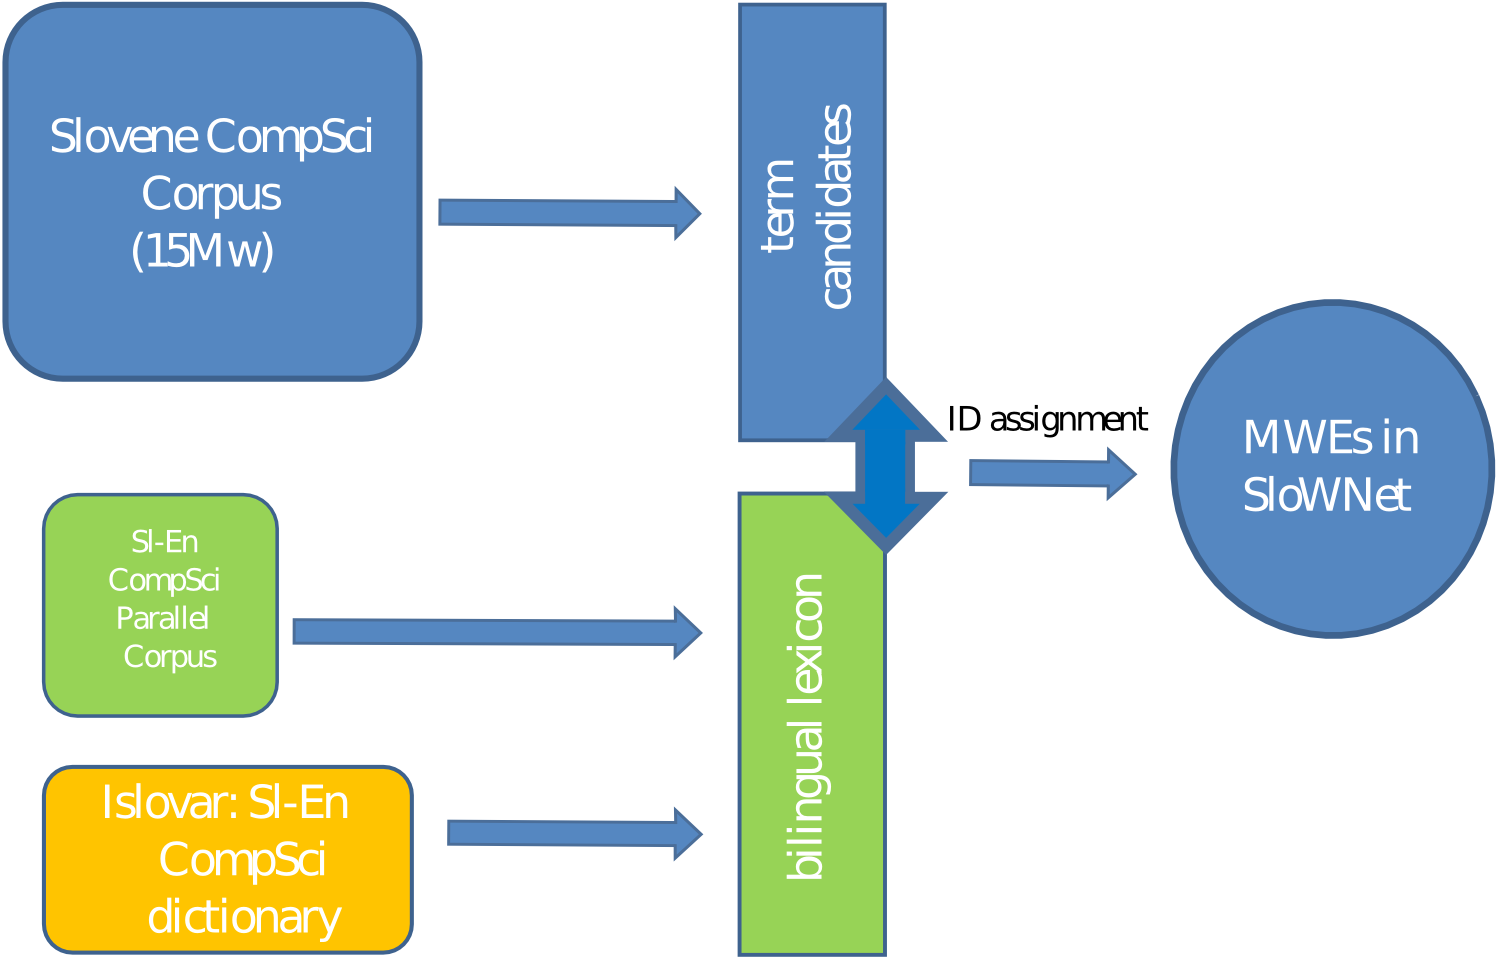
\includegraphics[width=\textwidth]{figures/VintarFiserF1a.png}
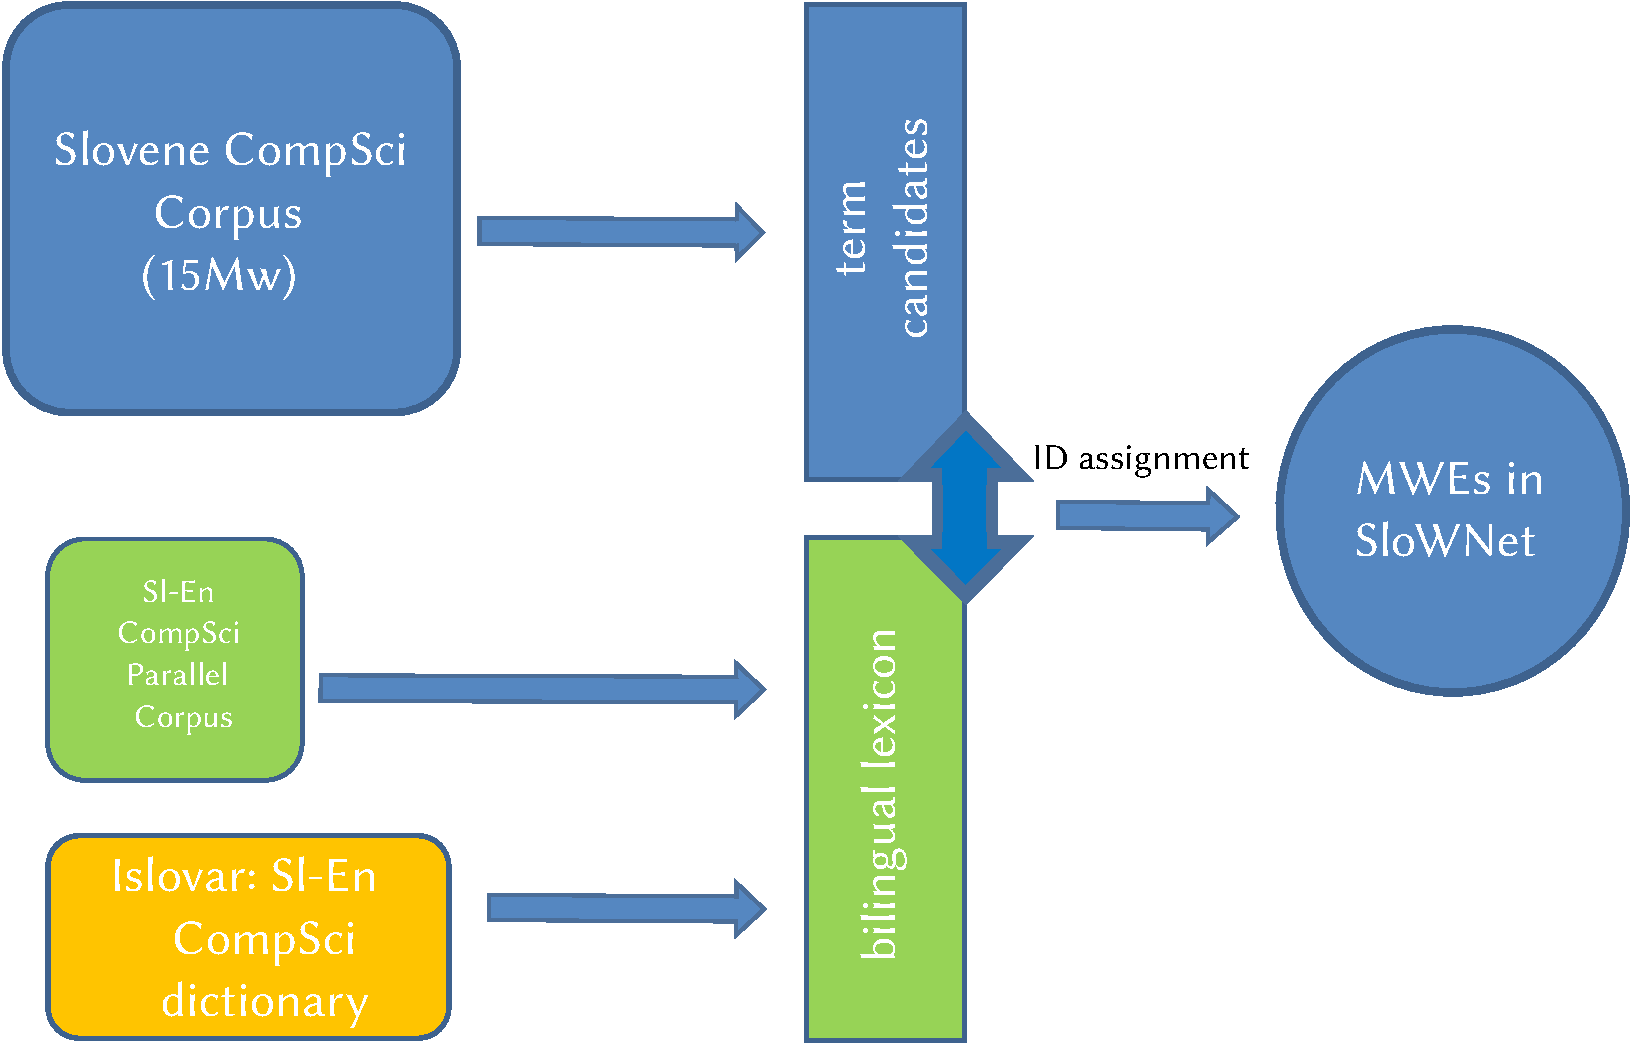
\includegraphics[width=\textwidth]{figures/VintarFiserF1.pdf}
\caption{Resources for harvesting MWEs}
\label{fig:vintar:1}
\end{figure}

\subsection{Automatic Term Extraction}\label{sec:vintar:3.3}

The domain-specific Ikorpus is composed of texts from five journals dealing with computer science, information and communication technology, and it also contains five consecutive volumes of proceedings of the largest informatics conference in Slovenia (DSI). Its size is approximately 15 million running words, which makes it an excellent and fairly representative source of \isi{terminology}.

The task of automatically identifying domain-specific terms in texts has been addressed by numefrom PWN 2.0 into Slovenerous authors and has been tackled to the extent that there now exist several commercial tools with \isi{term extraction} functionality. The main approaches described in literature range from statistical ones, where terms are viewed as kinds of collocations, and the challenge lies in identifying the optimal word dependency measure \citep{Dunning1993, Daille1995}, to more linguistically informed and hybrid approaches, where part-of-speech, morphology and syntax are exploited as indicators of \isi{termhood} (\citealt{Heid1999}; \citealt{DiasEtAl2000}). More recent approaches introduce semantics and utilize context features to detect terminologically relevant phrases in running text (\citealt{Maynard1999}; \citealt{Gillam2007}), as well as propose methods for the identification of term variants \citep{Jacquemin2001}. An overview of the trends is given in \citet{KageuraEtAl2004}. 

In our experiment, automatic \isi{term extraction} is performed using a hybrid approach based on morphosyntactic patterns for Slovene and statistical ranking of candidates \citep{Vintar2004, Vintar2009}. The patterns, such as Adjective+Noun or Noun+Noun[Gen], yield numerous potential MWEs. After candidate phrases are extracted from the corpora, a term weighting measure is used to assign a ``\isi{termhood}'' value to each phrase. The \isi{termhood} value $W$ of a candidate term $a$ consisting of $n$ words is computed as 

% \begin{equation}
% \ea
$$
{W(a)=\frac{f_{{a}}^{{2}}}{n}\ast \overset{{n}}{\underset{{1}}{\sum }}{(\text{log}\frac{f_{{n,D}}}{N_{{D}}}}-\text{log}\frac{f_{{n,R}}}{N_{{R}}})}
$$
% \z
% \end{equation}\\

\noindent where $f_a$ is the absolute frequency of the candidate term in the \isi{domain-specific corpus}, $f_{n,D}$ and $f_{n,R}$ are the frequencies of each constituent word in the domain-specific and the general language reference corpus respectively and $N_D$ and $N_R$ are the sizes of these two corpora in tokens. 

The rationale of the \isi{termhood} measure is that terms are composed of terminologically relevant words, and the measure of terminological relevance is the comparison of a word's frequency between a \isi{domain-specific corpus} and a general language corpus. This intuitive notion was first exploited by \citet{AhmadEtAl1992} and implemented in other \isi{term extraction} tasks \citep{Scott1998, HeidEtAl2001}, however mostly for single-word terms. We use a modified version of this idea by adjusting it to \isi{multi-word} expressions and including the frequency of the entire expression to override non-terminological phrases occurring only once. 

For example, if we compare two phrases a and b, both occurring in the corpus of computer science texts, \textit{spletni brskalnik} `web browser', (517) and \textit{kakovost izdelka} `product quality' (74), using the 619-million-words FidaPlus corpus as the source of comparative frequencies we get the following result which indicates that the first phrase is terminologically more relevant than the second:

\ea
\label{vintarfiser:ex:a}
W(a) = 517\textsuperscript{2}/2 * (9.18 + 2.93) = 1618434.89
\z

\ea
\label{vintarfiser:ex:b}
W(b) = 74\textsuperscript{2}/2 * (1.31 + 1.20) = 6872.38
\z

The \isi{term extraction} procedure performed on the 15-million-token Slovene corpus of computer science yielded over 70,000 term candidates of length up to 4 words (\tabref{tab:vintar:3}). Given this bulk we can safely assume that not all of them are really terms we would like to include in sloWNet. As it turns out, the candidates list contains a large number of named entities, such as names of software and hardware products, vendors and manufacturers. Since few of these names might be terminologically relevant, we excluded them from further processing. We also employed a frequency threshold and discarded all term candidates which occurred less than 5 times. 

The extractor uses morphosyntactic patterns, therefore each \isi{multi-word} \isi{term candidate}, e.g. \textit{domenski strežnik} `domain name server', can be automatically assigned a headword (\textit{strežnik} `server') and we assume this to be the \isi{hypernym} of the \isi{term candidate}. 

\begin{table}
\begin{tabular}{lr}
\lsptoprule
{\bfseries MWE size } & \bfseries Number of candidates \\
\midrule
2 words (Adj+N, N+N, ...) & 54,844 \\
3 words (Adj + Adj + N, N + Prep + N, ...) &  16,861 \\
4 words (Adj + Adj + N + N, ...) & 2,605 \\
\bfseries Total & \bfseries 74,310 \\
\lspbottomrule
\end{tabular}
\caption{Term candidates and their length in words}
\label{tab:vintar:3}
\end{table}

Clearly, the domain-specific terms constitute a valuable lexical resource, but not until we can introduce some semantic structure. The next step therefore is to integrate at least some of these terms into sloWNet.

\section{Mapping terms to sloWNet}\label{sec:vintar:4}

At this point we have a large number of Slovene \isi{multi-word} terms without any semantic information other than the headword of each unit. Thus, for a term such as \textit{prosto programje} `free software', since it has been extracted through the syntactic pattern Adjective + Noun, we know that \textit{programje} `software' is the headword and \textit{prosto} the modifier. We may also assume that \textit{programje} is the \isi{hypernym} of \textit{prosto programje}, and hence we could add \textit{prosto programje} into sloWNet as the \isi{hyponym} of \textit{programje}, but only if sloWNet already contains the required headword \textit{programje}. 

For many \isi{multi-word} terms this turns out not to be the case, which is why we wish to add both the \isi{hypernym} and its extracted hyponyms to sloWNet in order to fill as many lexical gaps as possible. We use the Princeton WordNet (PWN) as the source of semantic structure, and to be able to link \isi{headwords} to this structure we use bilingual \isi{lexicon extraction}. 

\subsection{Bilingual lexicon extraction}\label{sec:vintar:4.1}

Bilingual \isi{lexicon extraction}, also known as \isi{word alignment}, is a statistical procedure where for each source word \textit{a} the algorithm computes the probabilities of all of its potential translation equivalents \textit{t}\textit{\textsubscript{1}}\textit{, t}\textit{\textsubscript{2}}\textit{, t}\textit{\textsubscript{n}} in the \isi{target language} \citep{Och2003}. The translation equivalents with the highest probability scores are then proposed as entries in the bilingual lexicon. Bilingual \isi{lexicon extraction} can only be performed on parallel corpora or bitexts. 

A small English-Slovene \isi{parallel corpus} of 300,000 tokens is fed to the Uplug word aligner \citep{Tiedemann2003}, which produces suggested translations for each word found in the corpus. To improve accuracy, we use only alignments of words that occur more than once and \isi{alignment} scores over 0.05. This yields a bilingual single-word lexicon of 1326 words, mostly nouns (\tabref{tab:vintar:4}). 

\begin{table}
\begin{tabular}{cllclc}
\lsptoprule
{\bfseries Freq} & \bfseries Score & \bfseries English & \bfseries POS & \bfseries Slovene & \bfseries POS\\
\midrule
\bfseries 4 & 0.058264988 & adaptability & n & prilagodljivost & n\\
\bfseries 8 & 0.100445189 & additional & a & dodaten & a\\
\bfseries 5 & 0.138443460 & agent & n & agent & n\\
\lspbottomrule
\end{tabular}
\caption{Sample entries in the bilingual lexicon}
\label{tab:vintar:4}
\end{table}

\newpage 
In order to improve coverage and accuracy, the automatically extracted bilingual lexicon is further enlarged with entries from the English-Slovene online dictionary of computer science Islovar. The dictionary provides approximately 5,000 bilingual entries and is consulted also in certain cases of ambiguous headword, as described below.

\subsection{Adding Terms to sloWNet}\label{sec:vintar:4.2}

For each Slovene \isi{multi-word} \isi{term candidate} we first identify its headword and assume that the headword is its \isi{hypernym}. Using our bilingual lexicon we translate the headword into English and retrieve its \isi{synset} IDs from PWN. If the headword turns out to be monosemous, the entire group of \isi{multi-word} terms with the same \isi{hypernym} can be added to sloWNet under the unique \isi{synset} ID (\tabref{tab:vintar:5}).


\begin{table}
\resizebox{\textwidth}{!}{
\begin{tabular}{lll}
\lsptoprule
Term candidates & Hypernym, English & Selected \isi{synset} ID\\
& translation and & {}\\
& possible \isi{synset} IDs & {}\\ 
\midrule
prosto programje (`free software') & programje = software & ENG20-06162514-n\\
priloženo programje (`attached software') & {} & {} \\
ustrezno programje (`appropriate software') 
&  ENG20-06162514-n & {}\\
novejše programje (`updated software') & computer\_science & {}\\
dodatno programje (`additional software') & {} & {}\\
vohunsko programje (`spyware') & {} & {} \\
\lspbottomrule
\end{tabular}
}
\caption{Monosemous headword}
\label{tab:vintar:5}
\end{table}

If the headword could be assigned several possible senses, we exploit the domain label in the wordnet, such as \textit{factotum, biology} etc. If one of the senses of the polysemous headword belongs to the domain Computer Science, then this sense is chosen (\tabref{tab:vintar:6}).

\begin{table}
\resizebox{\textwidth}{!}{
\begin{tabular}{lll}
\lsptoprule
Term candidates & Hypernym, English & Selected \isi{synset} ID\\
& translation and & {}\\
& possible \isi{synset} IDs & {}\\
\midrule
vgrajena tipkovnica (`built-in keyboard') & tipkovnica = {keyboard} & ENG20-03480332-n \\
brezžična tipkovnica (`wireless keyboard') & {} & {}\\
zaslonska tipkovnica (`monitor keyboard') & ENG20-03480198-n & {}\\
tipkovnica qwerty (`QWERTY keyboard') & computer\_science & {} \\
navidezna tipkovnica (`virtual keyboard') & {} & {}\\
miniaturna tipkovnica (`miniature keyboard') & ENG20-03480332-n & {}\\
zunanja tipkovnica (`external keyboard') & factotum & {}\\
zložljiva tipkovnica (`folding keyboard') & {} & {}\\
ergonomska tipkovnica (`ergonomic keyboard') & {} & {}\\
programska tipkovnica (`program keyboard') & {} & {}\\
slovenska tipkovnica (`Slovene keyboard') & {} & {}\\
modularna tipkovnica (`modular keyboard') & {} & {}\\
alfanumerična tipkovnica (`alphanumeric keyboard') & {} & {}\\
\lspbottomrule
\end{tabular}
}
\caption{Polysemous headword with CompSci domain}
\label{tab:vintar:6}
\end{table}

If the headword is already part of sloWNet, no \isi{disambiguation} is needed and the terms can be simply added as hyponyms to the existing Slovene \isi{hypernym}. Also, in some cases one of the extracted \isi{multi-word} terms was already in the Islovar dictionary. We can then use the English translation of the term to look up the correct \isi{hypernym} and \isi{synset} ID in PWN. 

Nevertheless there remain many cases where the polysemous headword does not belong to the CompSci domain in the wordnet and it is neither included in sloWNet or Islovar. In such cases the correct sense must be picked manually (\tabref{tab:vintar:7}). 

\begin{table}
\resizebox{\textwidth}{!}{
\begin{tabular}{lll}
\lsptoprule
Term candidates & Hypernym, English & Selected \isi{synset} ID\\
& translation and & {}\\
& possible \isi{synset} IDs & {}\\
\midrule
nalaganje gonilnikov (`loading drivers') & nalaganje = {loading} & to be selected manually\\
nalaganje podatkov (`loading data') & {} & {}\\
nalaganje programov (`software download') & ENG20-00671518-n & {}\\
nalaganje strani (`loading page') & factotum & {}\\
 & ENG20-13044298-n & {} \\
 & transport & {} \\
\lspbottomrule
\end{tabular}
}
\caption{Polysemous headword, ID to be selected manually}
\label{tab:vintar:7}
\end{table}

\section{Discussion}\label{sec:vintar:5}

Extracting terms from a large domain-specific Slovene corpus yields the bulk of 74,310 term candidates. We keep only those that occur more than five times and where the headword and its English translation can be identified with reasonable accuracy, and we disregard all names and terms that include names. Some of the remaining terms were already either in the Islovar dictionary or in sloWNet, however the large majority were new. \tabref{tab:vintar:8} shows the number of terms successfully added to sloWNet. 

\begin{table}
\begin{tabular}{lr}
\lsptoprule
\textbf{Category} & \textbf{Number of terms} \\
\midrule
Already in sloWNet & 29 \\
Already in PWN &  23 \\
Already in Islovar & 198 \\
New & 5150 \\
\textbf{Total} & \textbf{5400} \\
\lspbottomrule
\end{tabular}
\caption{Total term candidates added to sloWNet}
\label{tab:vintar:8}
\end{table}

The assumption that the headword of the \isi{multi-word} expression is at the same time the \isi{hypernym} of the term may seem daring, however we encountered very few examples where this is not the case. Within a random sample of 200 \isi{multi-word} terms we found 5 terms where the headword could not be considered an appropriate \isi{hypernym} of the term, for example a \textit{spletni portal} `web portal' is not a kind of \textit{portal} `portal'; \textit{portal} being an architectural term, and \textit{prostor na disku} `disk space' is not a kind of \textit{prostor} `space'; although both of these \isi{headwords} could be used elliptically in a computer science context to mean \textit{web portal} or \textit{disk space} respectively. 

As has been described in the previous section, the difficult part is determining the correct sense of the potentially polysemous headword. This ambiguity can of course affect a large number of terms, since -- as can be seen in \tabref{tab:vintar:6} -- several dozens of \isi{multi-word} terms share the same headword. While we use all the semantic information we can infer either from the domain label or the online dictionary, nearly half of all the \isi{headwords} need to be disambiguated manually (\tabref{tab:vintar:9}).

\begin{table}
\begin{tabular}{lr}
\lsptoprule
\textbf{Category} & \textbf{Number of headwords}\\
\midrule
Monosemous & 84\\
Headwords with CompSci domain & 35\\
Headwords already in sloWNet &  11\\
Headwords derived from MWE PWN & 6\\
To be picked manually & 136\\
\textbf{Total} & \textbf{272}\\
\lspbottomrule
\end{tabular}
\caption{Categories of headwords}
\label{tab:vintar:9}
\end{table}

In this respect our methodology could benefit significantly from additional context-based \isi{disambiguation} procedures. A possible approach would be to use the contexts of the polysemous \isi{headwords} and compute the semantic similarity between the relevant context words and each sense of the headword. The sense with the greatest semantic similarity to the context features is selected as the correct one. This is essentially a word \isi{disambiguation} task and various authors have proposed similarity measures based on the graph representation of \isi{wordnets} (e.g. \citealt{Leacock1998}; \citealt{Wu1994}; \citealt{AgirreEtAl2009}). In future experiments we plan to implement such methods for the selection of the correct sense.

Finally it should be noted that the domain labels in Princeton WordNet are sometimes illogical, too specific or not specific enough. If we for example explore the financial domain, there is no label [Finance], but we find three different domains for a related set of concepts: \textit{money} [Money], \textit{coin} [Money], \textit{bank} [Banking], \textit{account} [Banking], \textit{pay} [Economy]. This is clearly a problem for automatic text processing, because we cannot rely on the fact that semantically related lexical items share the same domain label in WordNet. On the other hand there exists a hierarchical structure of WordNet domains which was not taken into account in our experiments. It may be the case that some ambiguity issues could be better resolved using this hierarchy.

\section{Conclusions}\label{sec:vintar:6}

We described an approach to improve the \isi{domain coverage} of a wordnet by enriching it with semi-automatically extracted \isi{multi-word} terms. Our method utilizes a combination of mono- and bilingual resources. A large monolingual \isi{domain-specific corpus} is used as the source of \isi{terminology}, and a smaller \isi{parallel corpus} combined with a domain-specific dictionary is used to provide translation equivalents of \isi{headwords}. These are required in order to map the semantic structure of Princeton WordNet onto the Slovene term candidates and thus integrate them into sloWNet. 

Although the approach works well and yields many items of specialised vocabulary, the most difficult part is the selection of the correct sense with polysemous \isi{headwords}. In some cases the correct sense can be inferred from the domain label or from the dictionary, but in many cases this step still has to be performed manually. In the future we plan to implement a sense \isi{disambiguation} procedure based on semantic similarity.

It should be noted that an evaluation of monolingual \isi{term extraction} lies beyond the scope of this paper and is not addressed, although the quality of the term candidates clearly influences the results of the experiment described. Term extraction evaluation depends heavily on the target application, which means that the same system may perform very well in an information retrieval task and poorly in a dictionary-making task. Since the measure of terminological relevance relies on the comparison of relative frequencies between a domain-specific and a reference corpus, the \isi{term extraction} system performs better for highly specialised domains or, in other words, for terms that do not occur frequently in general language. Information science is in this respect not the ideal domain because IT-related topics are regularly discussed in general language media.

The proposed methodology can be extended to other domains, or indeed other languages. While we employ a specialised monolingual corpus, a bilingual corpus and a specialised bilingual dictionary, the cross-language part of the al\-go\-rithm is essentially suited to parallel corpora. Especially in domains -- or language pairs -- for which bilingual dictionaries are scarce it is often more viable to construct a small \isi{parallel corpus} and use the word-aligned bilingual lexicon to translate \isi{headwords}. While in other domains we could again exploit the domain labels in WordNet to disambiguate the headword, our methodology is less suitable for general language where polysemy is common and \isi{disambiguation} can only be performed with context-based methods.

An evaluation of the \isi{domain coverage} of sloWNet will be performed within a Machine Translation application. In the future we also plan to extend this approach to the extraction of definitions from domain-specific corpora using Machine Learning to distinguish between well-formed and not-well-formed definitions \citep{Fišer2010}.

{\sloppy 
\printbibliography[heading=subbibliography,notkeyword=this]
}
\end{document}

